\subsubsection{Verbindung des Displays mit der Platine}
Das Display verfügt auf der Rückseite über mehrere Anschlüsse, die mit einfachen Pinleisten mit der Platine verbunden wurden. Hierfür wurden folgende Signale angeschlossen: GND und VCC als Spannungsversorgung. SCL, SDA, RES und CS dienen als Pins für die Datenübertragung per I²C-Bus. Der CS-Pin dient der Unterscheidung der beiden I²C-Busse. (Chip-Select) Hier bekommt das Display die Anweisung, ob und wann es die Daten auf dem I²C-Bus verarbeiten soll.\\
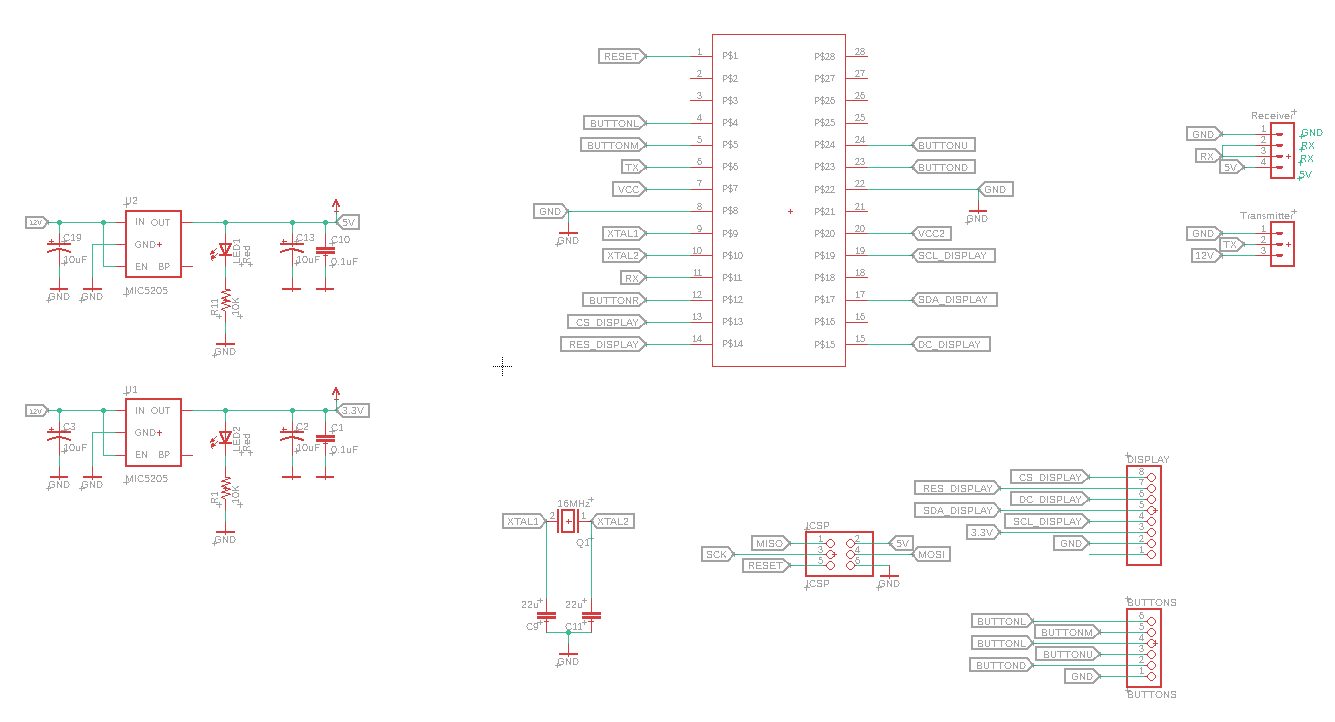
\includegraphics[width=\textwidth]{./Hauptteil/hw/schematic.png}